\section{{Resultados}}

Como se mencionó anteriormente, se realizaron dos instancias de experimentación.
En una primera instancia se consideraron únicamente antisacadas (N =
{first__starting_sample__subjects_count} sujetos) y en una segunda
instancia se incluyeron tanto antisacadas como prosacadas (N =
{second__starting_sample__subjects_count} sujetos).

\subsection{{Primera instancia}}

En la primera instancia se realizaron únicamente antisacadas. Se obtuvieron un
total de {first__starting_sample__trials_count} ensayos provenientes de
{first__starting_sample__subjects_count} sujetos.
Luego de aplicar el pre-procesamiento, la cantidad de ensayos se redujo a
{first__inlier_sample__trials_count} provenientes de
{first__inlier_sample__subjects_count} sujetos.
De estos, {first__correct_sample__trials_count} obtuvieron respuesta correcta y
{first__incorrect_sample__trials_count} obtuvieron respuesta incorrecta.
De las respuestas incorrectas, {first__corrected_sample__trials_count} tuvieron
una segunda sacada correctiva antes del fin del ensayo, es decir que tras mirar
al punto incorrecto, corrigió y realizó una sacada hacia el punto correcto.
Los ensayos correctos tuvieron un tiempo de respuesta mayor al de las
incorrectas (promedio $\pm$ desvio std: Correctas $=$ 
{first__correct_sample__mean_response_time} ms $\pm$ 
{first__correct_sample__stdev_response_time}; Incorrectas $=$
{first__incorrect_sample__mean_response_time} ms $\pm$
{first__incorrect_sample__stdev_response_time}).

\begin{{figure}}
  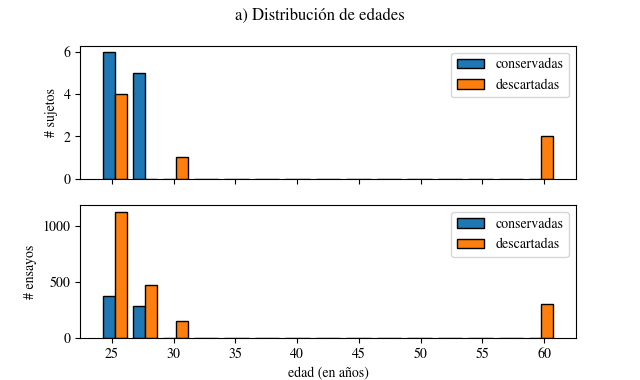
\includegraphics{{results/first-ages-distribution.png}}
  \caption{{Distribución de edades (primera instancia)}}
  \label{{fig:first-ages-distribution}}
\end{{figure}}

\begin{{figure}}
  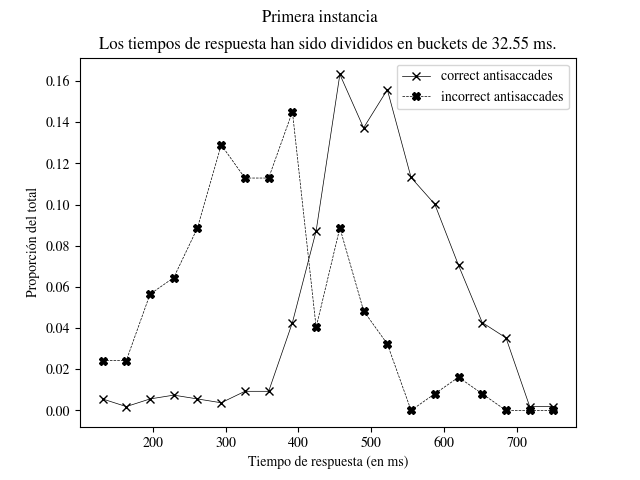
\includegraphics{{results/first-response-times-distribution.png}}
  \caption{{Distribución de tiempos de respuesta (primera instancia)}}
  \label{{fig:first-response-times-distribution}}
\end{{figure}}

\begin{{figure}}
  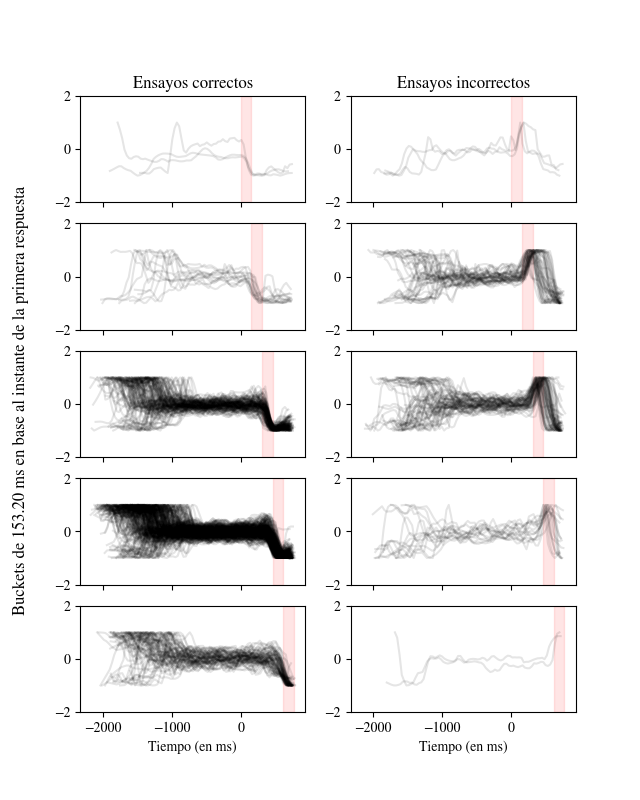
\includegraphics{{results/first-disaggregated-antisaccades.png}}
  \caption{{Antisacadas desagregadas (primera instancia)}}
  \label{{fig:first-disaggregated-prosaccades}}
\end{{figure}}

\subsubsection{{Estimaciones desviadas}} \label{{section:skewed-estimates}}

Se encontró que para varios sujetos [TODO: cuántos sujetos? con qué magnitud?]
las estimaciones obtenidas estaban desviadas del centro (Figura
\ref{{fig:skewed-estimations-example}}).
Para cada sujeto, estas desviaciones fueron consistentes a lo largo de todo el
experimento.
Además se mantuvo la posición relativa de las estimaciones.
Luego de ser apropiadamente normalizados, se logró entonces utilizar los datos
recolectados para identificar si la mirada caía en algunas de las tres regiones
de interés.

\begin{{figure}}
  \centering

  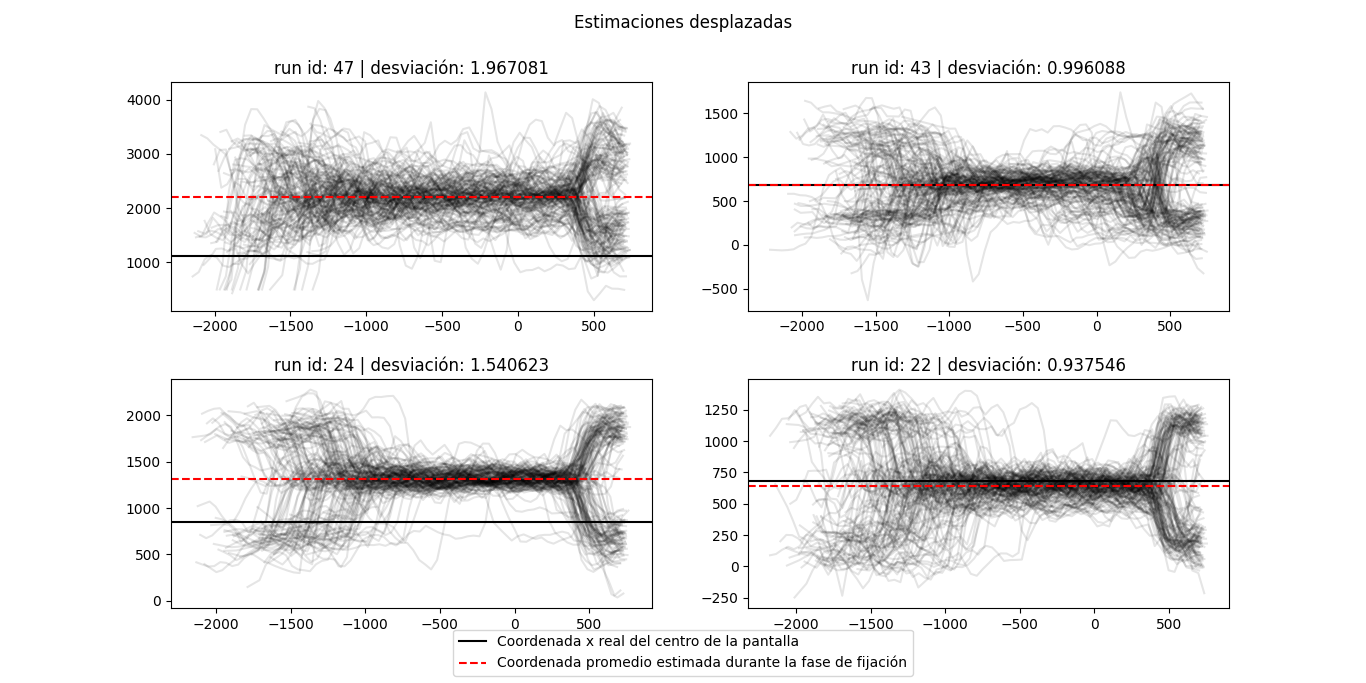
\includegraphics[width=\textwidth]{{results/skewed-estimations.png}}
  Durante la fase de fijación los sujetos 47 y 24 obtuvieron respectivamente
  estimaciones cercanas a los 2100 y 1400 píxeles, cuando los valores reales
  serían 1100 y 900.
  Estas desviaciones no ocurrieron para todo sujeto, como lo muestran los
  sujetos 42 y 22. \\
  El valor de desviación reportado [TODO: cambiar cómo se reporta esto que
  mucho no se entiende así como está] se calcula como la división entre la
  coordenada estimada del centro (el promedio de las estimaciones durante el
  período de fijación) y la coordenada real del centro.

  [TODO: Regenerar este plot para que macheen las dimensiones]

  \caption{{Ejemplos de sujetos con estimaciones desviadas}}
  \label{{fig:skewed-estimations-example}}
\end{{figure}}

\subsection{{Segunda instancia}}

Se obtuvieron un total de {second__starting_sample__trials_count} ensayos
provenientes de {second__starting_sample__subjects_count} sujetos.
{second__early_subjects_count} de estos tomaron la decisión de cortar
tempranamente el experimento.
Luego del preprocesamiento se terminó con {second__inlier_sample__trials_count}
ensayos provenientes de {second__inlier_sample__subjects_count} sujetos.
Para los ensayos válidos se obtuvo en promedio una correctitud de 
{second__prosaccades_correctness_percentage}$\%$ para la tarea de prosacadas y
de {second__antisaccades_correctness_percentage}$\%$ para aquella de
antisacadas.

\begin{{table}}[htb]
    \centering

              || anti            || pro             \\
              || corr   | incorr || corr   | incorr \\
        mean
          || {second__correct_antisaccades_sample__mean_response_time}
          | {second__incorrect_antisaccades_sample__mean_response_time}
          || {second__correct_prosaccades_sample__mean_response_time}
          | {second__incorrect_prosaccades_sample__mean_response_time} \\
        stdev
          || {second__correct_antisaccades_sample__stdev_response_time}
          | {second__incorrect_antisaccades_sample__stdev_response_time}
          || {second__correct_prosaccades_sample__stdev_response_time}
          | {second__incorrect_prosaccades_sample__stdev_response_time}

    \caption{{Tiempos de respuesta según correctitud y tarea}}
\end{{table}}

En un {second__antisaccades_correction_percentage}$\%$ de las antisacadas
incorrectos se realizó una corrección.
Tal corrección tomó en promedio
{second__corrected_antisaccades_sample__mean_correction_delay} ms (stdev
{second__corrected_antisaccades_sample__stdev_correction_delay} ms).


Para ambas tareas la categoría incorrecta presenta baja representatividad.
Luego de aplicar las reglas de filtrado se cuenta en total con
{second__incorrect_prosaccades_sample__trials_count} ensayos de prosacadas
incorrectas y {second__incorrect_antisaccades_sample__trials_count} ensayos de
antisacadas incorrectas.
En promedio cada sujeto termina con
{second__mean_incorrect_prosaccades_count_per_subject} ensayos de prosacadas
incorrectas y {second__mean_incorrect_antisaccades_count_per_subject}
ensayos de antisacadas incorrectas (cf. Tabla \ref{{tab:correctness}}).
Estas cantidades no significativas de ensayos imposibilitan analizar tiempos
obtenidos individualmente.
En futuras instancias de experimentación se deberá aumentar la cantidad de
ensayos inicial, tal que queden suficientes ensayos luego del
pre-procesamiento.
También se podrían revisar los criterios de exclusión de ensayos durante el
pre-procesamiento para asegurarse de que no se están descartando ensayos
válidos.

{second__correctness_summary_table}

\begin{{figure}}
  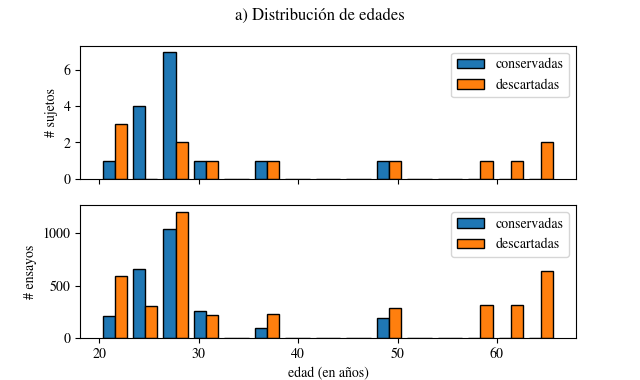
\includegraphics{{results/second-ages-distribution.png}}
  \caption{{Distribución de edades (segunda instancia)}}
  \label{{fig:second-ages-distribution}}
\end{{figure}}

\begin{{figure}}
  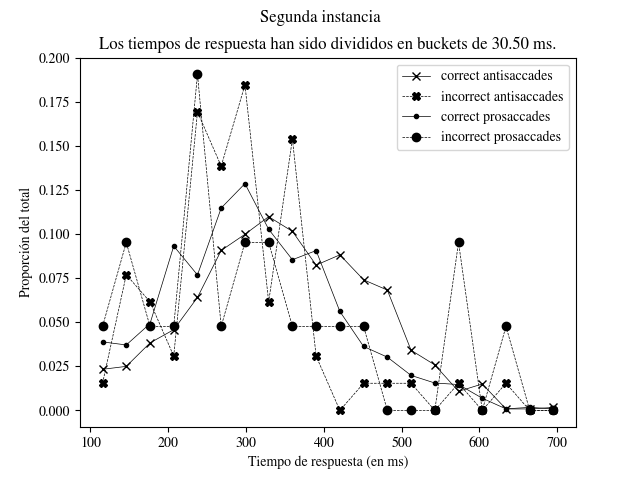
\includegraphics{{results/second-response-times-distribution.png}}
  \caption{{Distribución de tiempos de respuesta (segunda instancia)}}
  \label{{fig:second-response-times-distribution}}
\end{{figure}}

\begin{{figure}}
  \centering
  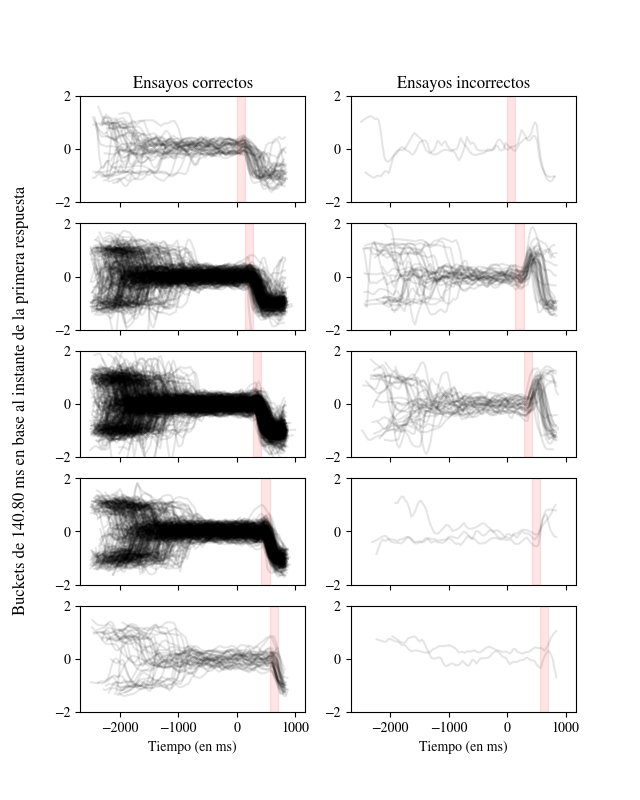
\includegraphics{{results/second-disaggregated-antisaccades.png}}
  \caption{{Antisacadas desagregadas (segunda instancia)}}
  [TODO: \\
  - Acá estaba explicando comentando que los datos estaban normalizados pero la
  verdad que no aporta.
  Sí comentar sobre los datos alineados temporalmente el efecto de la
  normalización en la \textit{{apariencia}} final de los datos.
  Lo mismo para la figura de prosacadas y para la de la primera instancia.
  Capaz se las pueda unificar y hacer en simultáneo comentario de las tres.]
  \label{{fig:second-disaggregated-antisaccades}}
\end{{figure}}

\begin{{figure}}
  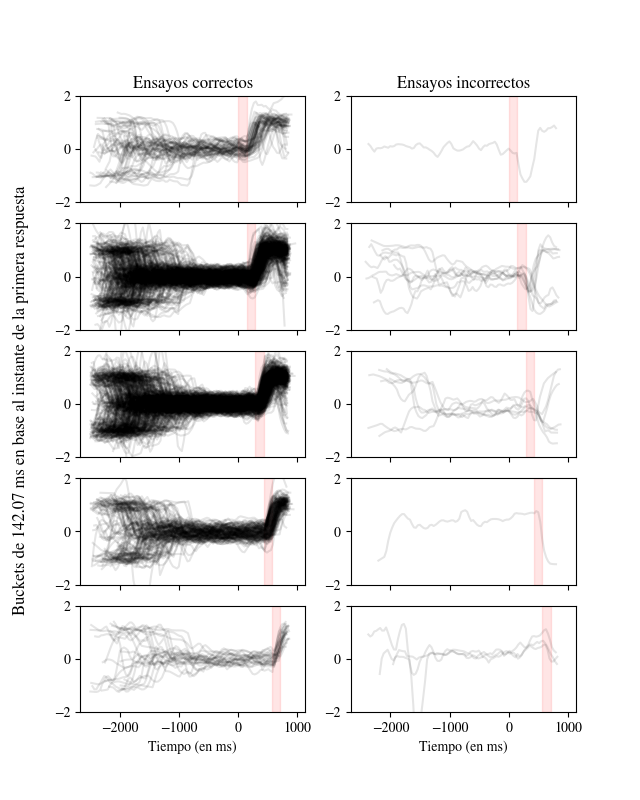
\includegraphics{{results/second-disaggregated-prosaccades.png}}
  \caption{{Prosacadas desagregadas (segunda instancia)}}
  \label{{fig:second-disaggregated-prosaccades}}
\end{{figure}}

\begin{{figure}}
  \centering
  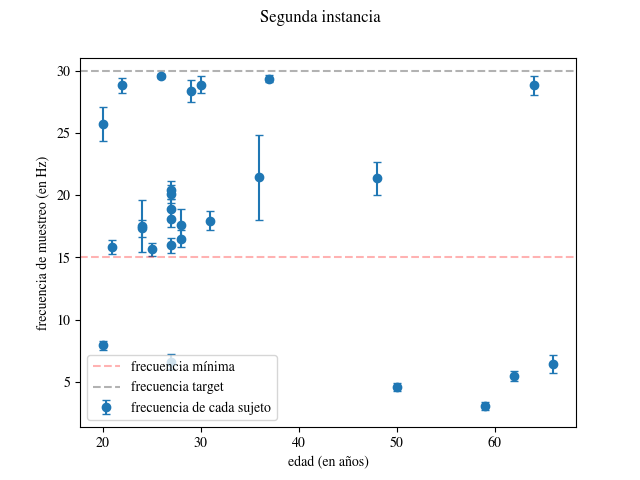
\includegraphics[width=\textwidth]{{
    results/second-sampling-frequencies-by-age.png}}
  \caption{{Frecuencia de muestreo en función de la edad}}
  [TODO: \\
  - Regenerar plot y ajustar dimensiones \\
  - Debería escribir algún comentario acá?]
  \label{{fig:sampling-frequencies-by-age}}
\end{{figure}}
